
\section{Method}


\begin{figure*}[t]
  \centering
  \makebox[\textwidth][c]{%
  \begin{minipage}[t]{0.29\textwidth}
    \centering
    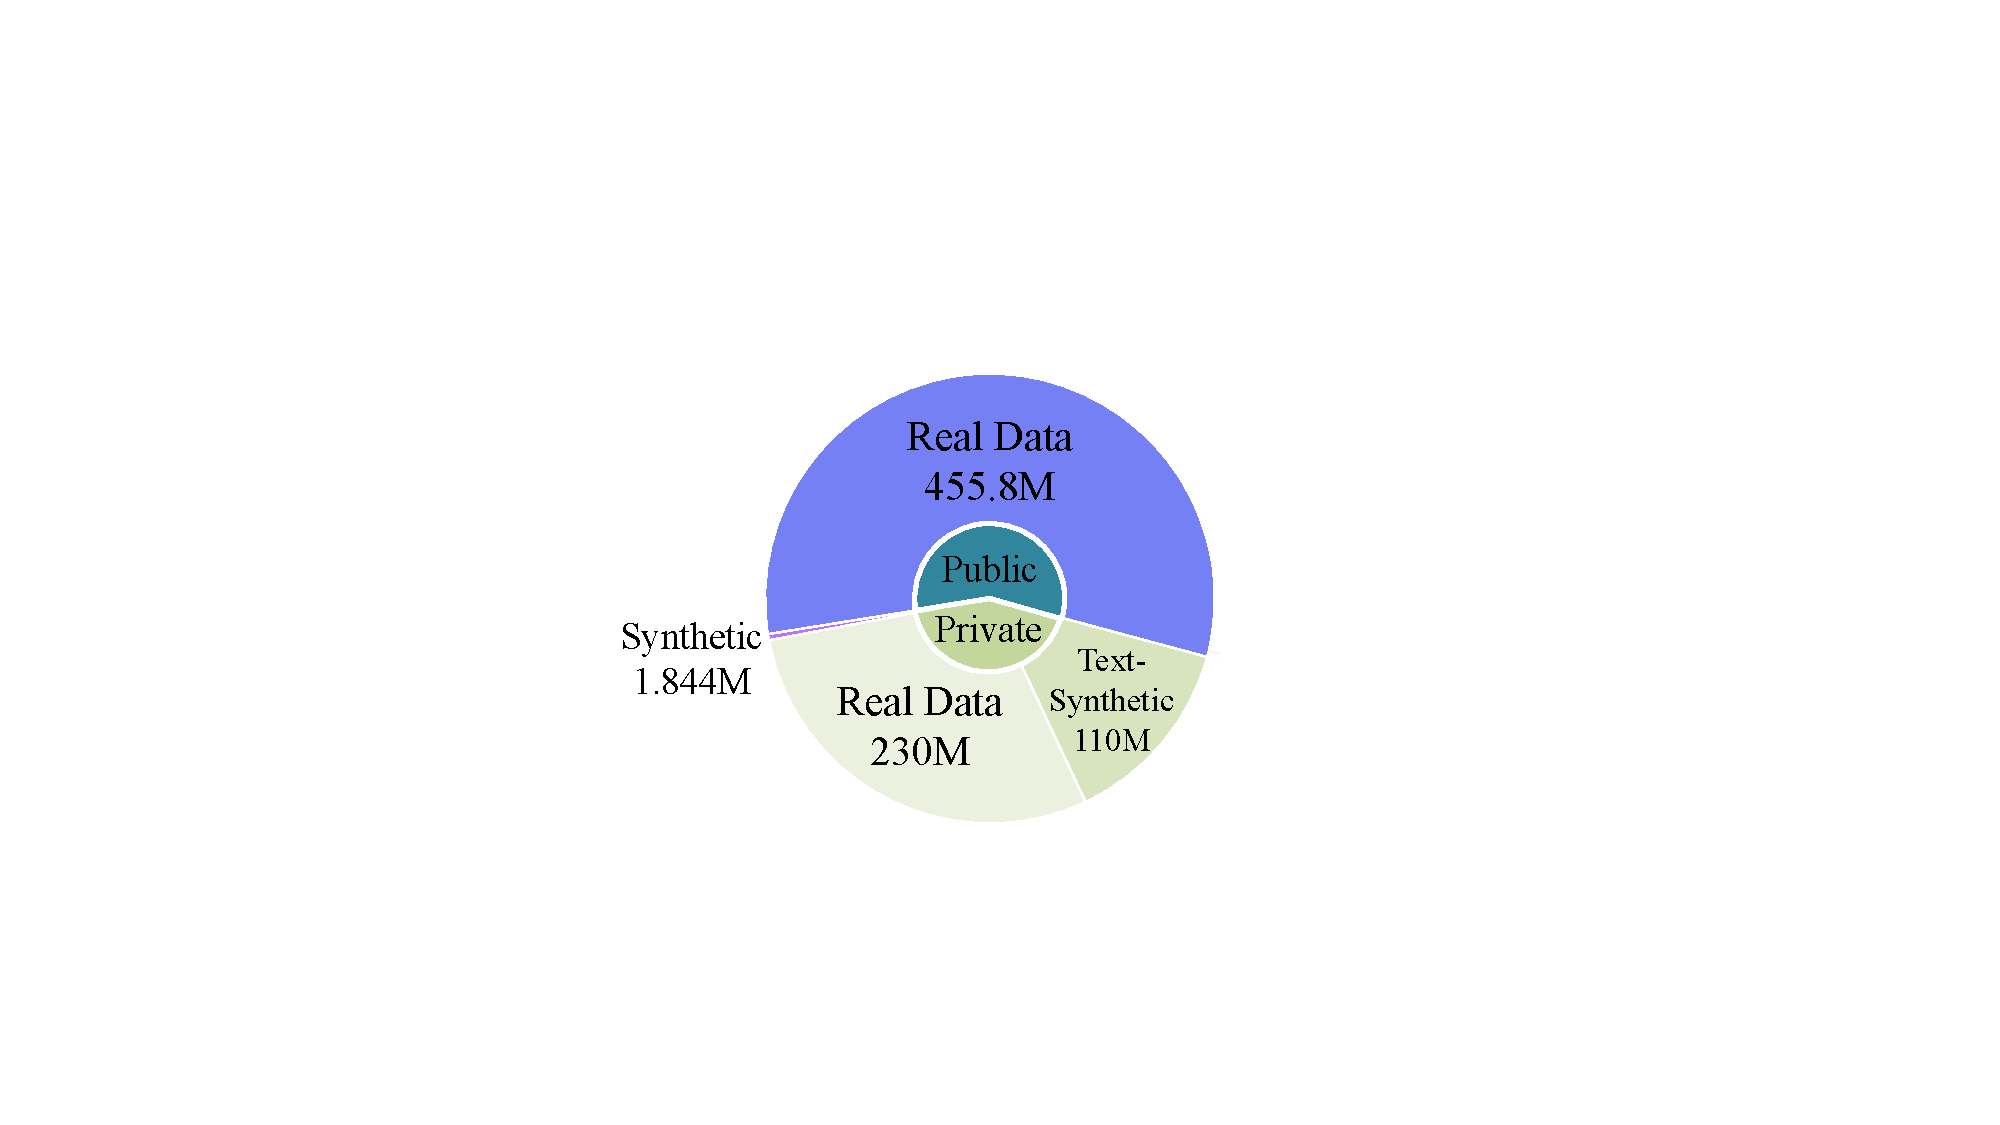
\includegraphics[width=\linewidth]{figures/Pre-training-Data.pdf}
    \\[-0.05em]
    \small (a) Lens-800M.
  \end{minipage}
  \hspace{0.001\textwidth}
  \begin{minipage}[t]{0.3\textwidth}
    \centering
    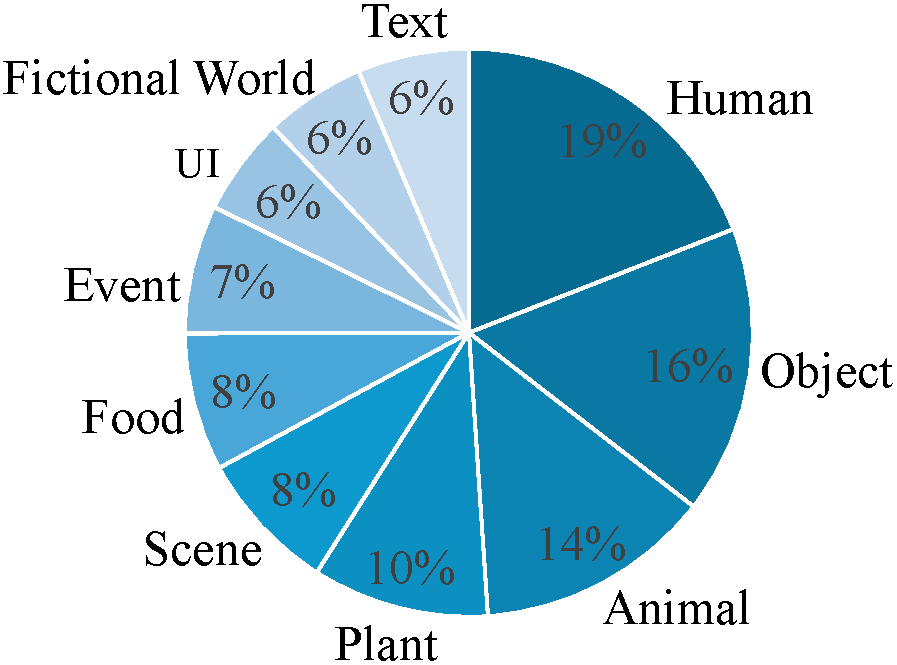
\includegraphics[width=\linewidth]{figures/RL-Data.pdf}
    \\[-0.05em]
    \small (b) Lens-RL-8K.
  \end{minipage}%
  \hspace{0.001\textwidth}
  \begin{minipage}[t]{0.38\textwidth}
    \centering
    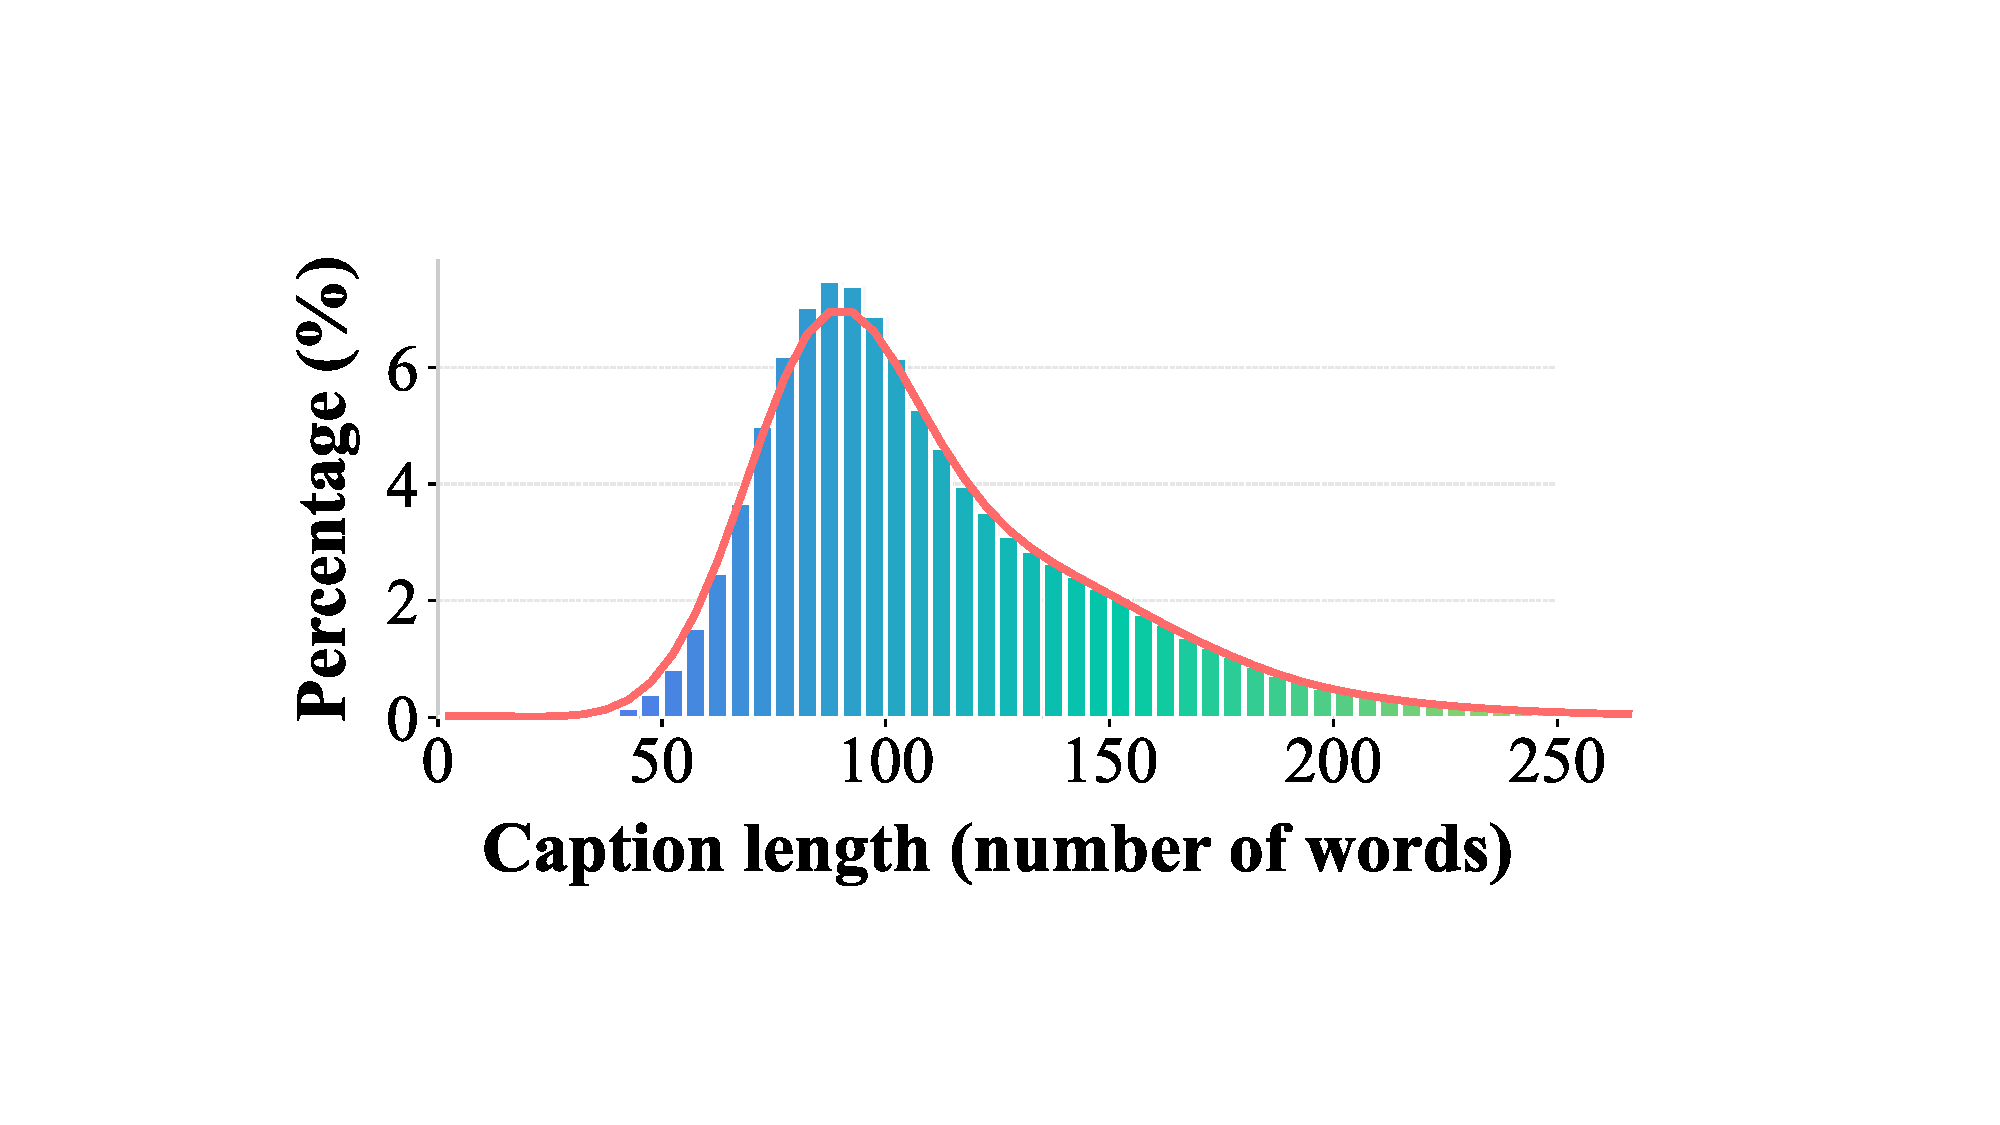
\includegraphics[width=\linewidth]{figures/Caption-length.pdf}
    \\[-0.05em]
    \small (c) Lens-800M.
  \end{minipage}%
  }
  %\vspace{-2mm}
  \caption{Distribution of (a) the pre-training dataset, \textit{Lens-800M}, (b) the RL dataset, \textit{Lens-RL-8K}, and (c) caption length distribution of the \textit{Lens-800M} dataset, caption length is measured by the number of words, with an average length of approximately 109 words.}
  %\vspace{-3mm}
  \label{fig:data-distribution}
\end{figure*}




In this section, we present the details of \textit{Lens}. We first describe the construction of the training dataset, \textit{Lens-800M}, in Section~\ref{sec:data}. We then present the model architecture in Section~\ref{sec:archi}, followed by the pre-training recipe in Section~\ref{sec:pre-training}. In Section~\ref{sec:post-training}, we introduce our RL-driven post-training strategy, which is built on the carefully designed \textit{Lens-RL-8K} dataset and optimized reward rubrics. We further introduce few-step distillation to distill \textit{Lens} into \textit{Lens-Turbo}, a 4-step generator that does not require CFG. Finally, Section~\ref{sec:optimization} discusses inference configuration and training-free system-prompt search.





\begin{figure}[t]
    \centering
    \begin{minipage}[t]{0.55\linewidth}
    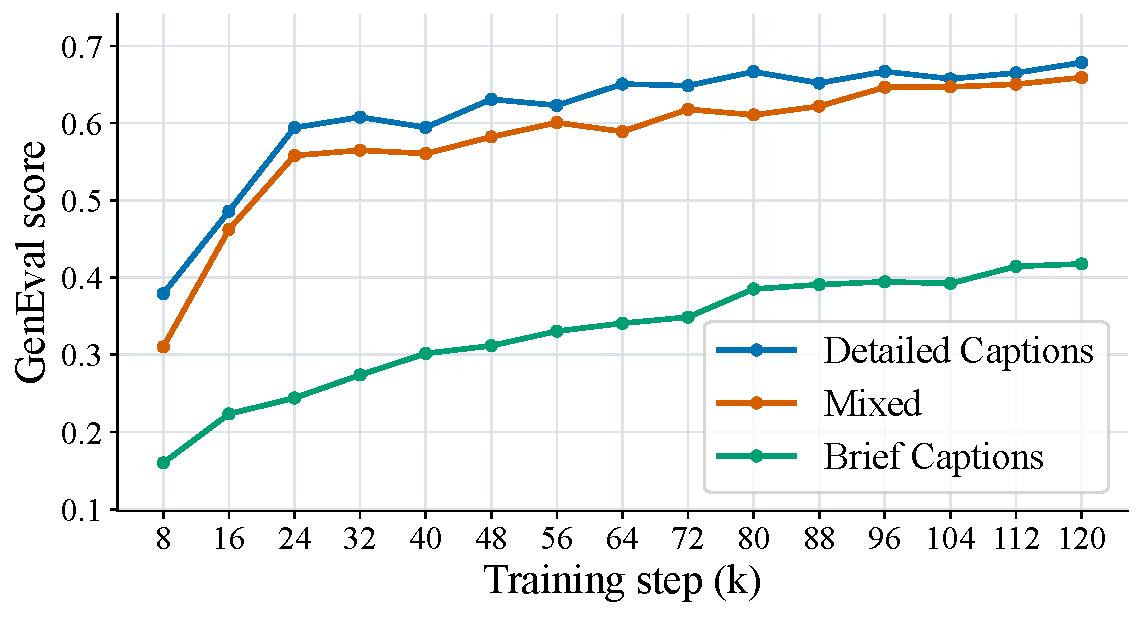
\includegraphics[width=1.0\linewidth]{figures/abl_caption.pdf}
    \vspace{-18pt}
    \caption{Caption-length ablation study.}
    \label{fig:abl_caption}
    \end{minipage}
\hfill
    \begin{minipage}[t]{0.44\linewidth}
    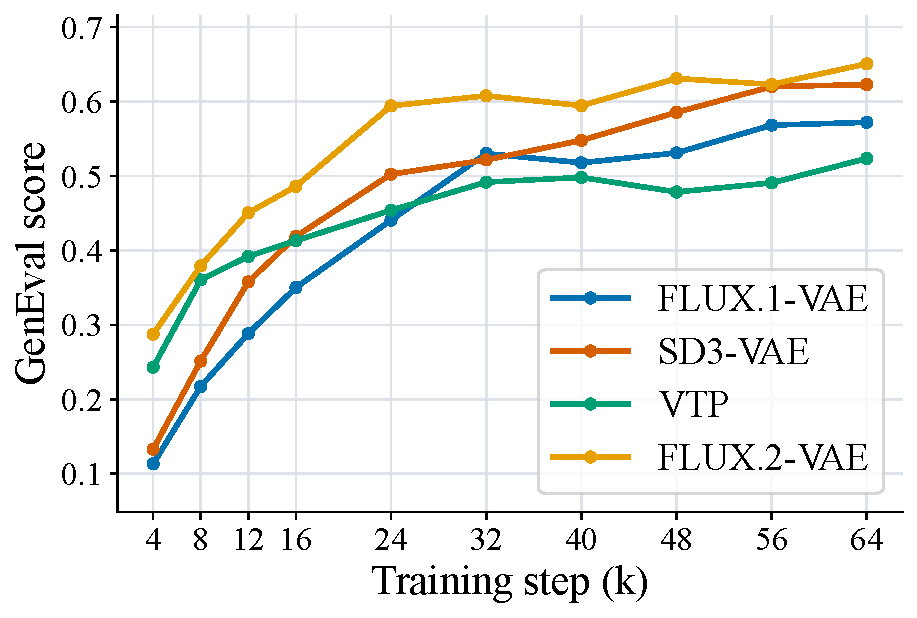
\includegraphics[width=1.0\linewidth]{figures/abl_vae.pdf}
    \vspace{-18pt}
    \caption{Ablation study on VAE variants.}
    \label{fig:abl_vae}
    \end{minipage}
    \vspace{-10pt}
\end{figure}


\subsection{Pre-training Data: Lens-800M}
\label{sec:data}

\noindent\textbf{Data Distribution.}
Our pre-training corpus is constructed from four complementary sources to ensure content diversity: \textit{(1) public real-world data}; \textit{(2) public synthetic data}; \textit{(3) private data}, covering text-heavy visual content such as posters, slides, graphic designs, and general-domain images; and \textit{(4) text synthetic data}, where text is rendered onto randomly sampled backgrounds with augmentations in blur, color, font, scale, and rotation to increase typographic and layout diversity. 

We apply a multi-stage data-cleaning pipeline to ensure the quality of the \textit{Lens-800M} pre-training dataset:
(1) removing corrupted or broken files;
(2) resolution filtering, where images with an area smaller than $384^2$ are removed;
(3) NSFW content filtering using an EVA model~\citep{freepik2025nsfw} fine-tuned for NSFW classification;
(4) aesthetic filtering using Aesthetic Predictor v2.5~\citep{schuhmann2022laion}, where samples with scores below 3 are discarded;
(5) watermark filtering using a SigLIP2 model~\citep{tschannen2025siglip} fine-tuned for watermark detection;
(6) clarity filtering, where visually blurry samples are removed based on the variance of the Laplacian computed on scale-normalized grayscale images;
(7) entropy filtering, where low-information samples are removed based on the Shannon entropy of grayscale intensity histograms;
(8) luminance filtering, where under- or over-exposed samples are removed based on the mean V-channel value in HSV color space, normalized to $[0,1]$;
and (9) near-duplicate removal using CLIP ViT-L/14 embeddings with a cosine-similarity threshold of $>0.985$, accelerated by FAISS~\citep{douze2024faiss, johnson2019billion} indexing.

After the data filtering process, the final pre-training dataset contains approximately \textit{800M} high-quality images. The detailed data distribution is illustrated in Figure~\ref{fig:data-distribution}(a). We refer to this pre-training dataset as \textbf{Lens-800M}.








\noindent\textbf{Captioning Images with Detailed Captions.}
For each image in \textit{Lens-800M}, we employ a strong vision-language model, GPT-4.1 in our implementation, to generate a detailed, long-form \textit{English} caption using the prompt described in Appendix~\ref{sec:prompt-caption}. At the same time, to preserve multilingual rendering capabilities, any text appearing in the image is kept in its original language in the caption. Figure~\ref{fig:data-distribution}(c) presents the caption length statistics. Training examples are provided in Appendix~\ref{sec:lens-800M visualization}.




This design is motivated by three considerations.
(1) \textit{Improving data quality.} Web-crawled alt-text captions are often short, underspecified, and sometimes incorrect. Such noisy supervision forces the model to resolve ambiguity during training, leading to inefficient capacity usage and degraded learning signals~\citep{betker2023improving,chen2024sharegpt4v}.
(2) \textit{Bridging the training–inference gap.} In real-world usage, users frequently provide long and compositional prompts to describe desired images. Training on detailed captions better aligns the model with this inference-time distribution.
(3) \textit{Enhancing data efficiency.} Empirically, we observe that training \emph{exclusively} on dense captions yields the best generation performance, outperforming short-caption training.

\noindent\textbf{Ablation Study: Detailed vs. Brief Captions.}
To validate observation (3), we conduct a controlled ablation study. We randomly sample 130M images from the \textit{Lens-800M} dataset to construct an ablation subset, denoted as \textbf{Lens-130M}. We train three small text-to-image models (referred to as \textbf{Lens-Toy}) with identical architectures (described in Section~\ref{sec:archi}), each using a 1.2B-parameter image generation backbone and a Qwen3-0.6B text encoder. The only difference lies in the captioning strategy:
\textit{(i) Brief}: where GPT-4.1 generates short and sparse captions (e.g., ``a photo of a cat'') for each image in \textit{Lens-130M};
\textit{(ii) Detailed}, which uses our generated dense captions; and \textit{(iii) Mixed}, a 50/50 combination of Brief and Detailed captions. We evaluate generation performance on the GenEval~\citep{ghosh2023geneval} benchmark. As shown in Figure~\ref{fig:abl_caption}, training with dense captions achieves better generation quality than the other variants, owing to improved data utilization efficiency.
 


\begin{tcolorbox}[colback=gray!5,colframe=black]
\textit{Dense caption supervision improves the data information density of each training batch, leading to better data utilization and higher training efficiency.}
\end{tcolorbox}


\subsection{Architecture}
\label{sec:archi}

Our model mainly consists of: (1) a \textit{VAE} that encodes images into compact latents; (2) a \textit{Latent Diffusion Transformer} that denoises text-conditioned image latents; (3) a \textit{Reasoner} that converts ambiguous user requests into detailed, well-formed prompts.




\noindent\textbf{VAE.} We examine both classical VAEs, including those used in FLUX.1~\citep{flux2024} and SD3~\citep{esser2024scaling}, and semantic VAEs, including those used in FLUX.2~\citep{flux-2-2025} and VTP~\citep{vtp}. We do not use rFID to evaluate VAE performance, since reconstruction fidelity mainly measures how well a VAE reproduces a given image, rather than how effectively its latent space supports generative learning. We also avoid relying on class-conditional ImageNet generation as a proxy evaluation. Instead, we directly assess each VAE in the text-to-image generation setting by training \textit{Lens-Toy} models on the \textit{Lens-130M} dataset introduced in Section~\ref{sec:data}. As shown in Figure~\ref{fig:abl_vae}, FLUX.2's VAE achieves the best generation performance while also accelerating model convergence, and is therefore adopted as the VAE in \textit{Lens}.



\begin{tcolorbox}[colback=gray!5,colframe=black]
\textit{The VAE is crucial for both generation quality and model convergence. A strong VAE defines a more compact and semantically meaningful visual latent space, making text-image alignment easier to learn and reducing the number of optimization steps required for convergence.}
\end{tcolorbox}


\begin{figure}[t]
  \centering
  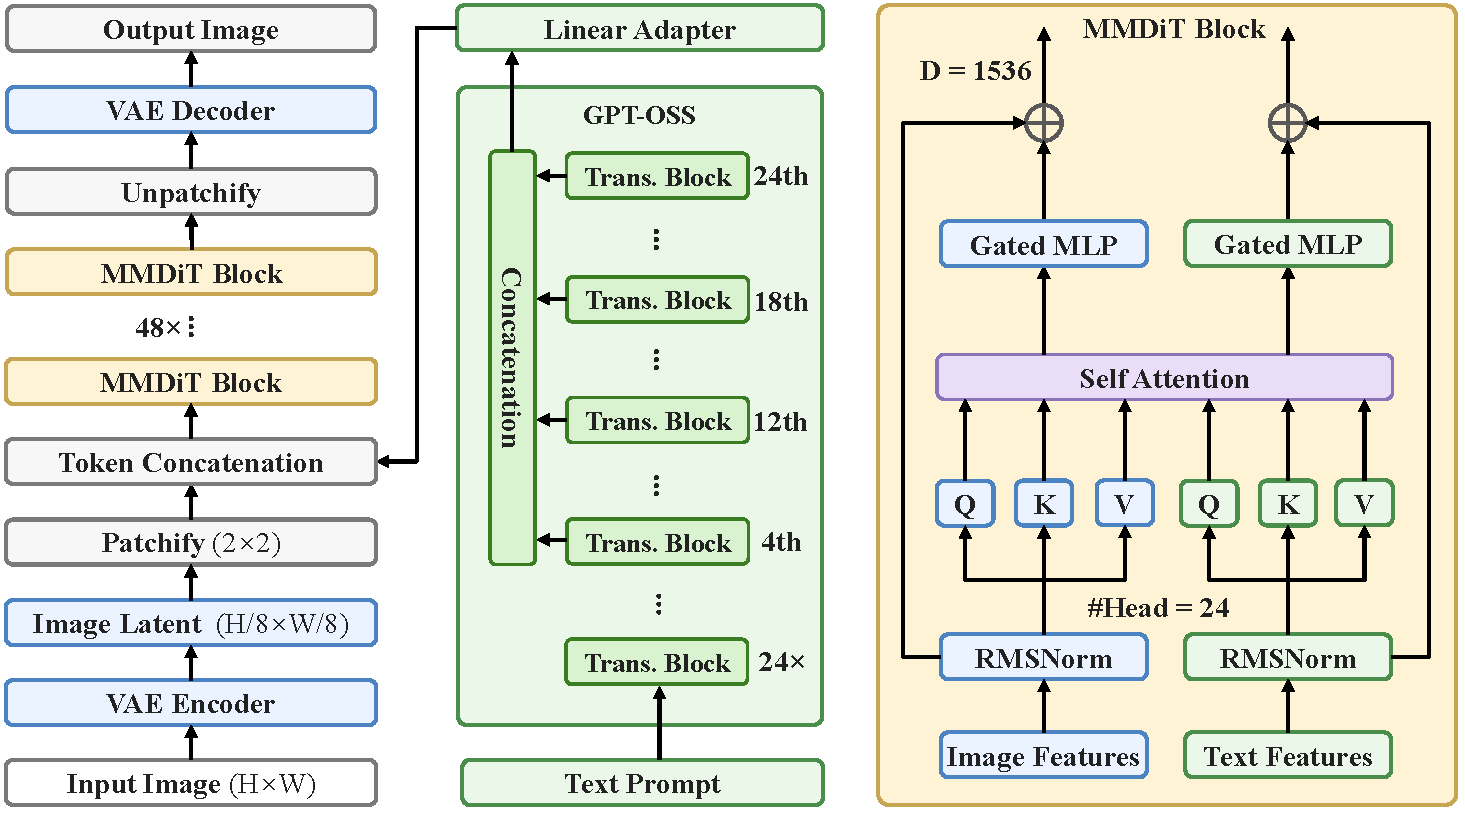
\includegraphics[width=\textwidth]{figures/Architecture.pdf}
 % \vspace{-6mm}
  \caption{Architecture of the latent diffusion Transformer in \textit{Lens} (left) and the detailed design of an MMDiT block (right). ``Trans.'': Transformer. }
  %\vspace{-3mm}
  \label{fig:architecture}
\end{figure}


\noindent\textbf{Latent Diffusion Transformer.}
We adopt an MMDiT-style~\citep{esser2024scaling} architecture for \textit{Lens}, as illustrated in Figure~\ref{fig:architecture}. \textit{Lens} is formulated as a latent diffusion model and trained with the standard flow-matching~\citep{lipman2023flow} objective. Image latents are extracted using the FLUX.2 VAE, while text features are obtained from GPT-OSS~\citep{openai2025gptoss120bgptoss20bmodel}, a 20B-parameter MoE language model with 3B activated parameters and 24 layers in total. To better leverage multi-level semantic representations, we extract GPT-OSS features from the 4th, 12th, 18th, and 24th layers and concatenate them along the feature dimension. A linear adapter is then applied to project the concatenated text representation into the same dimensionality as the image latents. The denoising backbone consists of 48 MMDiT blocks. Each block takes as input the concatenation of noisy image features and the text features produced by the previous MMDiT block, and processes them through two separate branches for image and text modalities. We use RMSNorm~\citep{zhang2019root} as the normalization layer and apply RoPE~\citep{su2024roformer} to the image features.




\noindent\textbf{Ablation Study: Language Encoder.}
We consider two key factors when selecting the language encoder: (1) whether a stronger language encoder can facilitate text-image alignment, leading to better generation performance and faster convergence; and (2) whether it can enable multilingual generalization, i.e., training on English-only image-text pairs while supporting inference in other languages. To verify these effects, we compare four language encoders: GPT-OSS (MoE, 20B-A3B)~\citep{openai2025gptoss120bgptoss20bmodel} and Qwen3~\citep{yang2025qwen3} with different model sizes, including 0.6B, 1.7B, and 4B. We use \textit{Lens-Toy} as the ablation model and construct four variants that differ only in the choice of language encoder. All variants are trained on \textit{Lens-130M}, which contains 130M image-text pairs with English-only captions. Figures~\ref{fig:abl_lang_eng} and~\ref{fig:abl_lang_multi} present performance curves on the GenEval~\citep{ghosh2023geneval} benchmark as a function of training iterations. Based on these results, we adopt GPT-OSS as our language encoder.

\begin{tcolorbox}[colback=gray!5,colframe=black]
\textit{Strong language encoders provide a richer semantic text space for text-image alignment, bringing three key benefits: improved prompt-following fidelity, faster model convergence, and, most importantly, support for multilingual inputs beyond the training language without additional multilingual image-text training data.}
\end{tcolorbox}



\begin{figure}[t]
    \centering
    \begin{minipage}[t]{0.49\linewidth}
    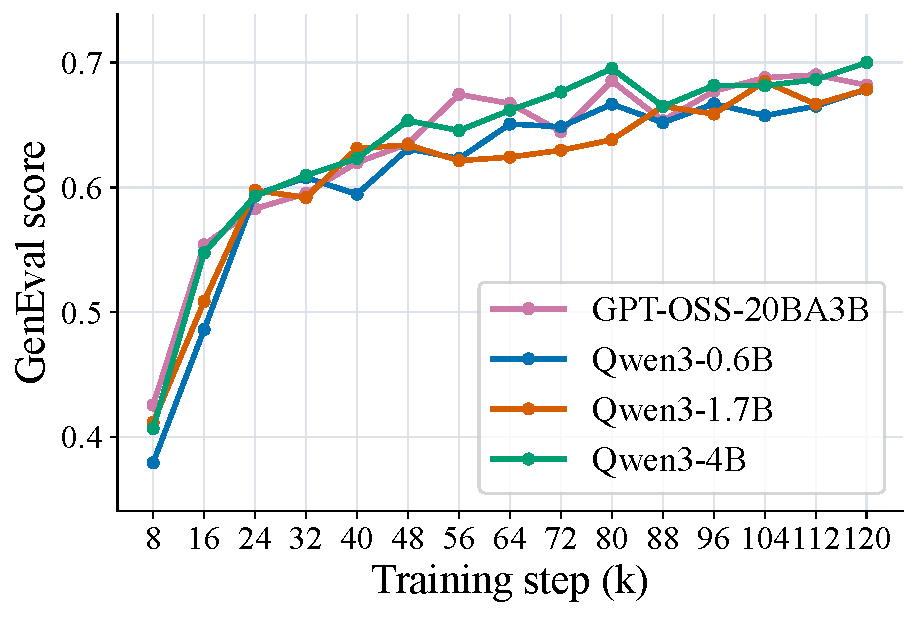
\includegraphics[width=1.0\linewidth]{figures/abl_lang_qwen3_english.pdf}
    \vspace{-17pt}
    \caption{Study of different language encoders for English text-conditioned generation.}
    \label{fig:abl_lang_eng}
    \end{minipage}
\hfill
    \begin{minipage}[t]{0.49\linewidth}
    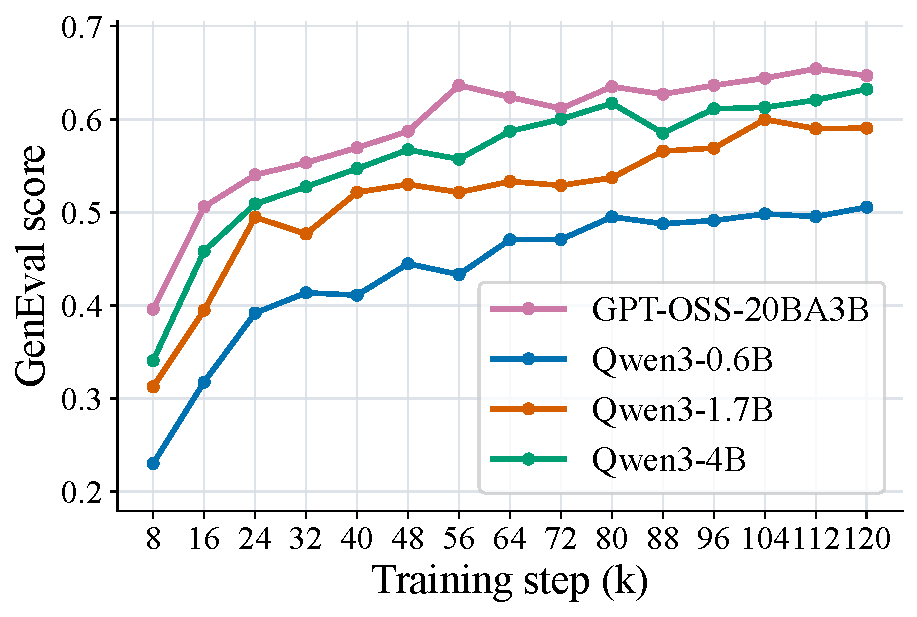
\includegraphics[width=1.0\linewidth]{figures/abl_lang_qwen3_avg5.pdf}
    \vspace{-17pt}
    \caption{Study of language encoders for multilingual text-conditioned generation, averaged over five common languages (EN/ZH/FR/JA/ES).}
    \label{fig:abl_lang_multi}
    \end{minipage}
    %\vspace{-3mm}
\end{figure}

\noindent\textbf{Reasoner.} The Reasoner is an independent language module placed before the T2I model. Its role is to interpret the user's raw input, refine ambiguous or underspecified instructions, and convert them into more detailed, coherent prompts optimized for generation. Because it functions independently of the T2I model's internal text encoder, the Reasoner can be easily swapped out without retraining the generation backbone. While we use GPT-5.5 as our default, the Reasoner is compatible with various commercial and open-source LLMs. Our evaluations in Appendix~\ref{sec:various reasoners} show that even using an open-source model like GPT-OSS provides substantial gains. This setup is particularly efficient: since GPT-OSS already functions as our text encoder, employing it as the Reasoner adds zero extra GPU memory cost, demonstrating that our framework can achieve superior results without relying on costly commercial APIs.






\subsection{Pre-training}
\label{sec:pre-training}


\noindent\textbf{Low-resolution Pre-training.} We first pre-train \textit{Lens} at a fixed resolution of $512\times512$ on 128 NVIDIA A100 80GB GPUs for 400K iterations. The FLUX.2 VAE and GPT-OSS language encoder are kept frozen, and only the diffusion transformer is optimized using the flow-matching MSE objective. We adopt logit-normal timestep sampling with $\mu{=}1.06$, corresponding to the 1024 image tokens of a $512\times512$ image. Training is performed in bfloat16 with gradient checkpointing. We use AdamW~\citep{loshchilov2019adamw} with $\beta_1{=}0.9$ and $\beta_2{=}0.999$, a constant learning rate of $2\times10^{-4}$, an effective global batch size of 3072 images, and gradient clipping set to 1.0.

\noindent\textbf{Mixed-resolution Continual Training.} Starting from the low-resolution checkpoint, we continue training for another 400K iterations using WebDataset bucket sampling over mixed resolutions on 128 NVIDIA A100 80GB GPUs. Specifically, we construct the resolution bucket set from three base image areas, $512^2$, $768^2$, and $1024^2$, combined with nine aspect ratios: $1{:}2$, $9{:}16$, $2{:}3$, $3{:}4$, $1{:}1$, $4{:}3$, $3{:}2$, $16{:}9$, and $2{:}1$. This results in 27 concrete resolution buckets: for the $512^2$ base, $352\times704$, $384\times672$, $416\times640$, $448\times608$, $512\times512$, $608\times448$, $640\times416$, $672\times384$, and $704\times352$; for the $768^2$ base, $544\times1088$, $576\times1024$, $640\times960$, $672\times896$, $768\times768$, $896\times672$, $960\times640$, $1024\times576$, and $1088\times544$; and for the $1024^2$ base, $736\times1472$, $768\times1376$, $832\times1248$, $864\times1152$, $1024\times1024$, $1152\times864$, $1248\times832$, $1376\times768$, and $1472\times736$.

For logit-normal timestep sampling, we adapt $\mu$ according to the image token length $n$: $\mu(n)$ is linearly interpolated from $\mu{=}1.0$ at $n{=}256$ tokens to $\mu{=}1.3$ at $n{=}4096$ tokens. We keep the same frozen VAE/language-encoder setup and optimizer as in low-resolution pre-training, and use per-base bucket batch sizes of 24, 10, and 6 for $512^2$, $768^2$, and $1024^2$, respectively. Since different ranks may process different resolutions within the same optimization step and high-resolution buckets require more computation, these resolution-dependent batch sizes are chosen to balance per-step wall-clock time across ranks. We train with a constant learning rate of $1\times10^{-4}$, while keeping the remaining optimizer configuration unchanged.



\noindent\textbf{Resolution and Aspect-ratio Generalization after Pre-training.}
Although the base model is trained on only 27 resolutions, constructed from 3 base areas and 9 aspect ratios, it generalizes well to unseen resolutions and aspect ratios at inference time. Specifically, it can generate images with arbitrary aspect ratios ranging from $1{:}2$ to $2{:}1$ and image areas up to $1440^2$, even though training does not include resolutions between $1024^2$ and $1440^2$, nor aspect ratios outside the predefined bucket set. This suggests that mixed-resolution pre-training does not simply encourage the model to memorize a fixed set of resolution buckets. Instead, exposure to diverse spatial scales and aspect ratios enables the model to learn more continuous and resolution-aware image representations. Moreover, the use of RoPE-based positional encoding may further facilitate such generalization, as it represents positions in a relative and extrapolatable manner.


\begin{tcolorbox}[colback=gray!5,colframe=black]
\textit{Mixed-resolution training enables strong resolution generalization at inference time, allowing the model to generate images at unseen sizes and diverse aspect ratios. This reduces the need to collect and train on images covering every target resolution and aspect-ratio combination. More importantly, since training on higher-resolution images increases computational cost quadratically with image size, resolution generalization allows the model to produce higher-resolution outputs while being trained primarily on lower-resolution images. This substantially reduces training cost and improves overall training efficiency.}
\end{tcolorbox}



\subsection{Post-training}
\label{sec:post-training}

After pre-training, our base model, \textit{Lens-Base}, can strictly follow user prompts and generate diverse images. However, the generated images may still contain visual artifacts. To further improve generation quality and reliability, we adopt reinforcement learning as a post-training strategy. 



\noindent\textbf{Lens-RL-8K Dataset.} \textit{Lens-RL-8K} is a prompt dataset designed for RL-based post-training, consisting of $8{,}406$ prompts that cover a broad range of T2I generation scenarios. A key observation in this work is that RL prompts should match the generation-scenario distribution of the pre-training data as comprehensively as possible. This enables post-training to improve the model’s overall generation quality and alignment across diverse scenarios, rather than overfitting to a narrow set of prompt types. 


We propose a taxonomy-driven construction pipeline for building the \textit{Lens-RL-8K} prompt set for RL training. First, we summarize common generation scenarios into a category set, including \texttt{Human}, \texttt{Object}, \texttt{Animal}, \texttt{Plant}, \texttt{Scene}, \texttt{Food}, \texttt{Event}, \texttt{Fictional World}, \texttt{Text}, and \texttt{UI and Graphic Design}. For each category, we further define dozens of fine-grained sub-categories. For example, the \texttt{Human} category includes sub-categories such as \texttt{Race}, \texttt{Occupation}, and \texttt{Gender}. Each sub-category then contains hundreds of concrete items. For instance, the \texttt{Race} sub-category includes items such as \texttt{White People} and \texttt{Asian People}, while the \texttt{Occupation} sub-category includes items such as \texttt{Researcher} and \texttt{Doctor}. In total, we construct an item set containing $8,406$ concrete items.


Next, we define a description set that specifies the key dimensions used to enrich each prompt, including \texttt{Attribute}, \texttt{Spatial Relationship}, \texttt{Count}, \texttt{Interaction}, and \texttt{Color}. These description dimensions provide basic guidance for generating diverse and detailed prompts for each concrete item.


Finally, for each item in the item set, we randomly sample one to four dimensions from the description set and prompt GPT-4.1 to generate an image-generation prompt using the system prompt detailed in Appendix~\ref{sec:prompt-lens-RL-8K}. This process yields $8,406$ RL prompts, forming the \textit{Lens-RL-8K} dataset. The category distribution of the prompts is shown in Figure~\ref{fig:data-distribution}(b).



\noindent\textbf{Rubric Generation.}
Rubrics define the key aspects used to assess images generated by \textit{Lens}. Given a prompt $\mathcal{P}$ from the \textit{Lens-RL-8K} dataset, we first generate 10 sample-aware rubrics using GPT-4.1. Specifically, we feed $\mathcal{P}$ together with the system prompt described in Appendix~\ref{sec:prompt-rubric} into GPT-4.1 to produce prompt-specific rubrics. We further append a global rubric, i.e., ``\textit{Verify that the entire image is structurally coherent and physically plausible}''. As a result, each prompt is associated with a set of evaluation rubrics. We also provide several prompt-rubric examples in Appendix~\ref{vis:rubric}.

\begin{table*}[t]
    \centering
    \vspace{-5mm}
    \caption{Left: Comparison of different \textit{Lens-RL} variants trained on different subsets of \textit{Lens-RL-8K} on GenEval. Right: Comparison between \textit{Lens-RL} models trained on the full \textit{Lens-RL-8K} set and a subset excluding text prompts on two text-rendering benchmarks, CVTG and OneIG (EN).}
    \vspace{-2mm}
    \label{tab:rl_diversity_ablation}

    \begin{tabular}{c@{\hspace{1mm}}c}
        {
        \renewcommand{\arraystretch}{1.06}
        \begin{tabular}[t]{lc}
            \toprule
            RL Training Set & GenEval \\
            \midrule
            1/4 Full set & 0.916 \\
            1/2 Full set & 0.920 \\
            Full set  & 0.930 \\
            \bottomrule
        \end{tabular}
        }
        &
        {
        \renewcommand{\arraystretch}{0.94}
        \begin{tabular}[t]{lcccc}
            \toprule
            \multirow{2}{*}{\raisebox{-0.6ex}{RL Training Set}} & \multicolumn{3}{c}{CVTG} & OneIG (EN) \\
            \cmidrule(r){2-4} \cmidrule(l){5-5}
             & Avg. & NED & CLIP & Text \\
            \midrule
            Full set \textit{w/o} text & 0.832 & 0.928 & 0.795 & 0.946 \\
            Full set  & 0.869 & 0.951 & 0.814 & 0.960 \\
            \bottomrule
        \end{tabular}
        }
    \end{tabular}
\end{table*}

\noindent\textbf{DiffusionNFT with VLM as Reward Function.}
We adopt DiffusionNFT~\citep{zheng2025diffusionnft} to optimize \textit{Lens-Base}, using GPT-4.1-mini as the reward function, inspired by RubricRL~\citep{feng2025rubricrl}. Specifically, at each optimization step, we randomly sample 48 prompt-rubric pairs and generate 24 images at different resolutions for each prompt using the current policy model. We then feed each generated image, together with its corresponding rubrics, into GPT-4.1-mini. Guided by the system prompt described in Appendix~\ref{sec:prompt-reward}, GPT-4.1-mini produces rewards that are used by DiffusionNFT to optimize the policy model. We train the RL policy for 180 steps on 64 NVIDIA A100 GPUs. Further details are provided in Appendix~\ref{sec:RL-Details}.



\noindent\textbf{Ablation Study: Various RL Datasets.} To verify that prompt diversity in the RL dataset is crucial for post-training performance, we conduct two ablation studies. First, we compare our default model, \textit{Lens-RL}, trained on the full \textit{Lens-RL-8K} dataset, with a variant trained on \textit{Lens-RL-8K} after removing text-related prompts. Second, we compare \textit{Lens-RL} with variants trained on smaller subsets of \textit{Lens-RL-8K}, including one-half and one-quarter of the full dataset, which substantially reduce the diversity of RL training prompts. All models are initialized from the same base model and trained for the same 180 RL steps. The results are reported in Table~\ref{tab:rl_diversity_ablation}.


\begin{tcolorbox}[colback=gray!5,colframe=black]
\textit{A broad and well-balanced RL prompt set enables the model to improve across diverse generation scenarios, whereas reduced or biased prompt coverage limits generalization.}
\end{tcolorbox}

\noindent\textbf{Few-step Distillation.} To improve sampling efficiency, we distill \textit{Lens-RL} into \textit{Lens-Turbo}, a 4-step generator distilled from a curated, well-balanced image-caption dataset. Our recipe combines effective techniques from DMD2~\citep{dmd2}, decoupled-DMD~\citep{decoupleddmd}, and SenseFlow~\citep{senseflow}, together with R1 regularization~\citep{R1penalty, apt} on the adversarial loss to improve training stability. \textit{Lens-Turbo} largely preserves the image quality and prompt-following ability of the original model. Details are provided in Appendix~\ref{sec:Distill-Details}.




\subsection{Inference}
\label{sec:optimization}



By default, we first use a reasoner to refine ambiguous or underspecified user inputs into more detailed prompts. The refined prompts are then fed into \textit{Lens} for \textbf{20}-step generation with CFG set to 5.0. For faster inference, \textit{Lens-Turbo} performs \textbf{4}-step generation without CFG.


\noindent\textbf{Training-free System-prompt Search.}
This technique aims to find a better system prompt for the reasoner, enabling it to more effectively convert user requests into suitable T2I model prompts. It requires no model training. Instead, we iteratively feed the previous system prompt and generation analysis, i.e., textual summaries of failure cases, into GPT-5.5, and ask it to rewrite the system prompt. We find that this training-free strategy produces improved system prompts for the reasoner. This strategy is not specific to our T2I system; it can also be applied to other T2I models.

